\documentclass{article}
\usepackage{amsmath, amsthm, amssymb, amsfonts, bm}
\usepackage{graphicx}
\usepackage[T1]{fontenc}
\usepackage[utf8]{inputenc}
\usepackage[a4paper]{geometry}
\usepackage{fancyhdr}
\usepackage[algo2e]{algorithm2e}
%\usepackage{verbatim}
%\usepackage{framed}
%\usepackage{fancyvrb}
%\usepackage[dvipsnames]{xcolor}  % colors
\fontfamily{cmr}

%% redefine \VerbatimInput
%\RecustomVerbatimCommand{\VerbatimInput}{VerbatimInput}%
%{fontsize=\tiny,
% %
% frame=lines,  % top and bottom rule only
% framesep=1em, % separation between frame and text
% rulecolor=\color{Black},
% %
% label=\fbox{\color{Black}Synthesized text},
% labelposition=topline,
% %
% commandchars=\|\(\), % escape character and argument delimiters for
%                      % commands within the verbatim
% commentchar=*        % comment character
%}

\title{DD2424 - Assignment 4 (Bonus)}
\author{Oskar Stigland \\ stigland@kth.se}

\pagestyle{fancy}
\fancyhf{}
\rhead{stigland@kth.se}
\lhead{DD2424 - Deep Learning in Data Science}
\rfoot{Page \thepage}

\begin{document}
%\maketitle

	\begin{titlepage}
		\begin{center} 
			
			\rule{\linewidth}{0.5mm}\\[0.5 cm]
			{ \huge \bfseries DD2424 - Assignment 4 (Bonus)}\\[0.3 cm] % Title of your document
			\rule{\linewidth}{0.5mm}\\[1 cm]
					
			\small\vfill
			\begin{center}
			\centering
			{\large \bfseries \textsc{Summary}}\\
			\vspace{1cm}
			\begin{minipage}{10cm}
				
				I have completed three of the four suggested bonus extensions, using \texttt{Adam} instead of \texttt{AdaGrad}, splitting the into chunks and randomizing them during training, and finally implementing temperature and nucleus sampling to attempt to generate more realistic text.\\\\
%
	The code for the assignment has been written in \texttt{python}. I have implemented the neural network as a class. For the hand-in, all of the code has been put toghether in a main file with all the functions and the class declared at the top. For the hand-in, I have also commented out the saving of generated figures and results in JSON files, as well as omitting some of the case-specific testing and gradient testing.
			\end{minipage}
			\end{center}
			\large\vfill
						

		\end{center}	
		
		\begin{minipage}{0.4\textwidth}
			\begin{flushleft} \large
				%\emph{Student:}\\
				Oskar \textsc{Stigland}\\
				DD2424\\
				Spring 2023
			\end{flushleft}
		\end{minipage}	

	\end{titlepage}

\newpage
\subsection*{\texttt{AdaGrad} versus \texttt{Adam}}
	I first ventured into testing the effect of replacing the \texttt{AdaGrad} optimizer with the much-popular \texttt{Adam}, for which we compute the updates as
	\begin{align*}
		\bm{w}_{k+1} &= \bm{w}_k - \eta\frac{\tilde{\bm{m}}_k}{\tilde{\bm{v}}_k + \epsilon} \\
		\tilde{\bm{m}}_k &= \bm{m}_k \times (1 - \beta_1^t + \epsilon)^{-1} \\
		\tilde{\bm{v}}_k &= \bm{v}_k \times (1 - \beta_2^t + \epsilon)^{-1} \\
		\bm{m}_k &= \beta_1^t \times \bm{m}_{k-1} + (1 - \beta_1^t)\times\nabla_{\bm{w}}L \\
		\bm{v}_k &= \beta_2^t \times \bm{v}_{k-1} + (1 - \beta_2^t) \times (\nabla_{\bm{w}}L)^2
	\end{align*}
	where $\epsilon$ is a very small numnber and $t$ is usually updated per training batch. Further, we have that $\beta_1 = 0.9$ and $\beta_2 = 0.999$. In this case, I have used $\eta = 0.01$ for \texttt{AdaGrad} and $\eta = 0.001$ for \texttt{Adam}, and since the data will be split into randomized chunks, $t$ is updated after each chunk, usually corresponding to some $500$ training examples. In order to properly check the effect of changing optimizer, I have also carved out the last $5$\% of the training examples for validation, and a smooth validation loss is tracked along with the smooth training loss. For the former, a random sample is selected after each training example and both smooth loss are then updated according to:
	    $$\tilde{\ell}^{\text{train}}_t = 0.999\times\tilde{\ell}^{\text{train}}_{t-1} + 0.001 \times\ell^{\text{train}}_{t}, \quad\text{and}\quad \tilde{\ell}^{\text{val}}_t = 0.999\times\tilde{\ell}^{\text{val}}_{t-1} + 0.001 \times\ell^{\text{val}}_{t}$$
	The difference in training performance when using \texttt{AdaGrad} and \texttt{Adam} is shown in the figure below.
	\begin{figure}[h!]
		\centering
		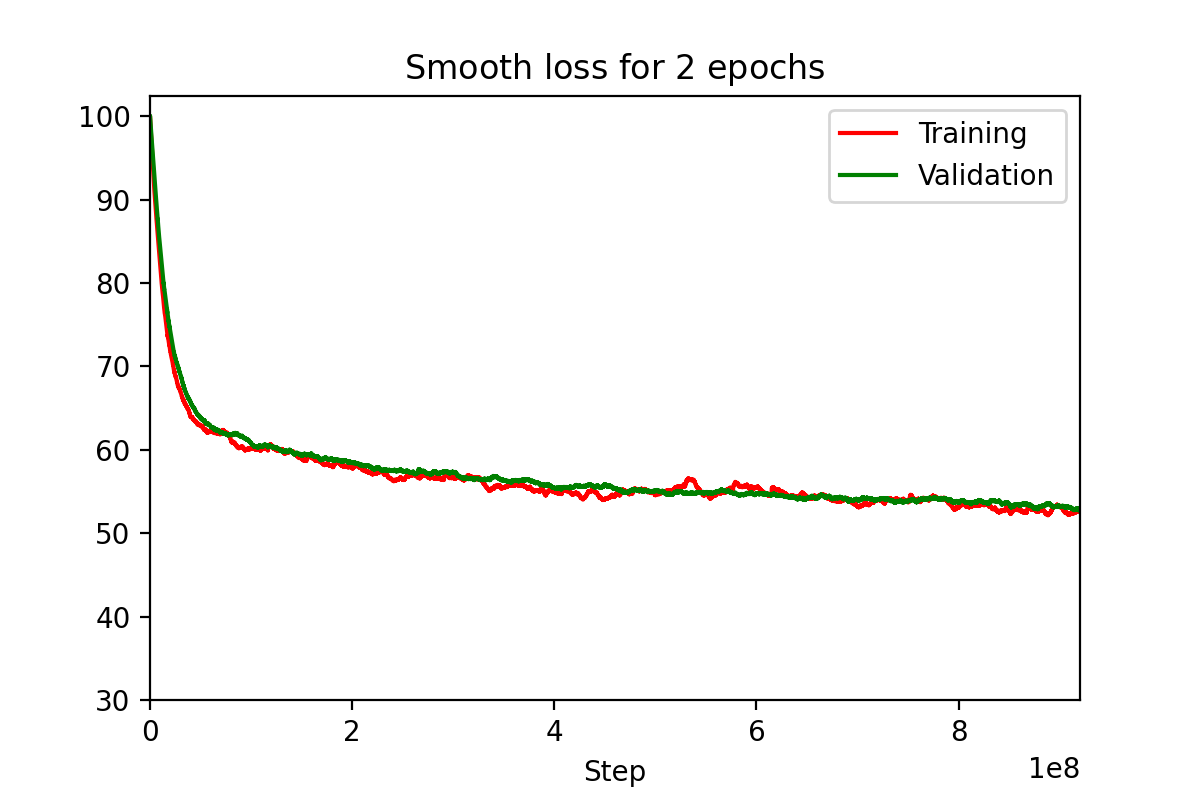
\includegraphics[width=7cm]{../plots/rnn_loss_v1.png}
		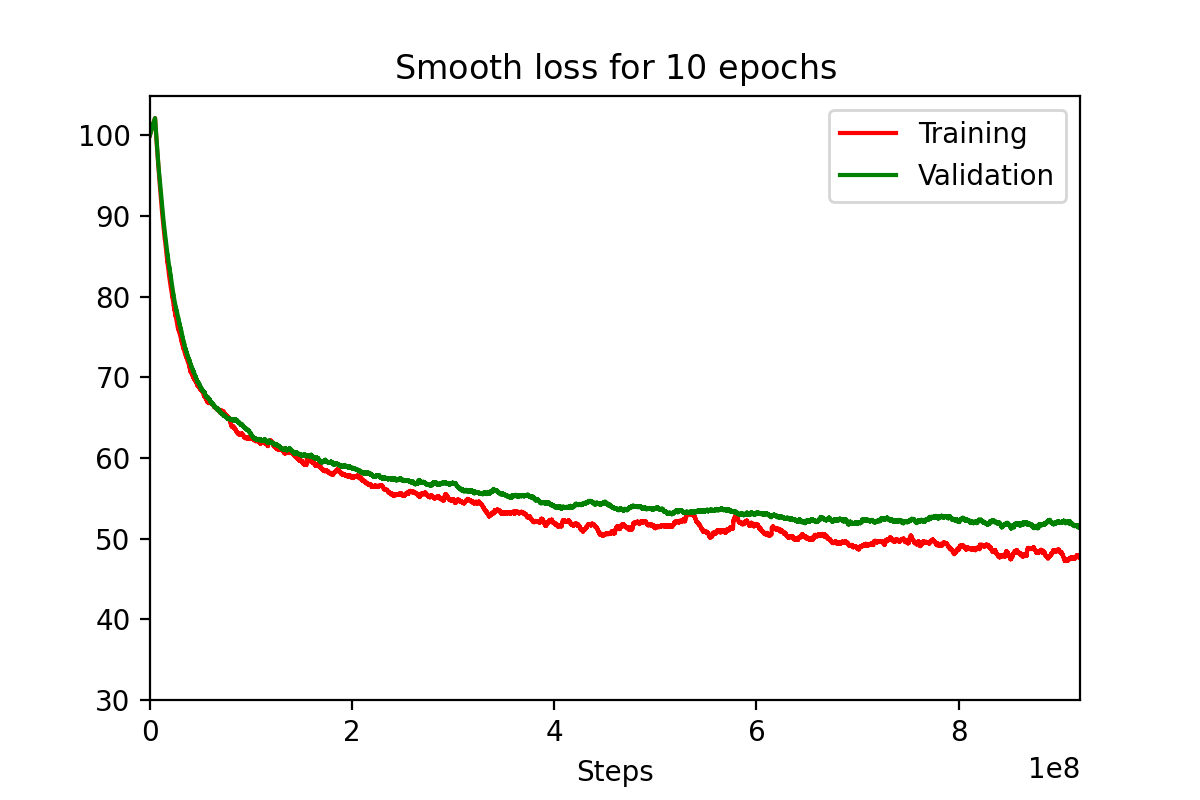
\includegraphics[width=7cm]{../plots/rnn_loss_v2.png}
		\caption{Training and validation loss for \texttt{AdaGrad} (left) and \texttt{Adam} (right), after $2$ epochs of training and $\eta = 0.01$.}
 	\end{figure}
	The performance for the two optimizers is very similar. However, \texttt{Adam} does seem to offer a slight improvement over \texttt{AdaGrad}. For the former, there also seems to be a slight gap between training and validation loss which also seems to become more pronounced as training goes on. Hence, it might be more prone to lead to an overfitting model in this particular case.
	
\newpage
\subsection*{Training with randomly ordered chunks}
	In the first experiment, the data was iterated through sequentially. However, this might introduce temporal dependencies, for example skewing the validation loss whenever we reach the end of an epoch (since the validation loss is extracted as the last $\sim5$\% of sequences. Instead, it seems more sensible to train on randomly selected sequences. This does, however, introduce the problem of memory and context and would require the $h_0$ to be reset at every training step. Thus, I split the data into $100$ blocks, save the last $5$ for validation and shuffle the rest at the beginning of each epoch, such that $h_0$ does not have to be reset at each training step - but instead only at the beginning of each block of training examples. The results are shown for both \texttt{AdaGrad} and \texttt{Adam} in the figure below.
	\begin{figure}[h!]
		\centering
		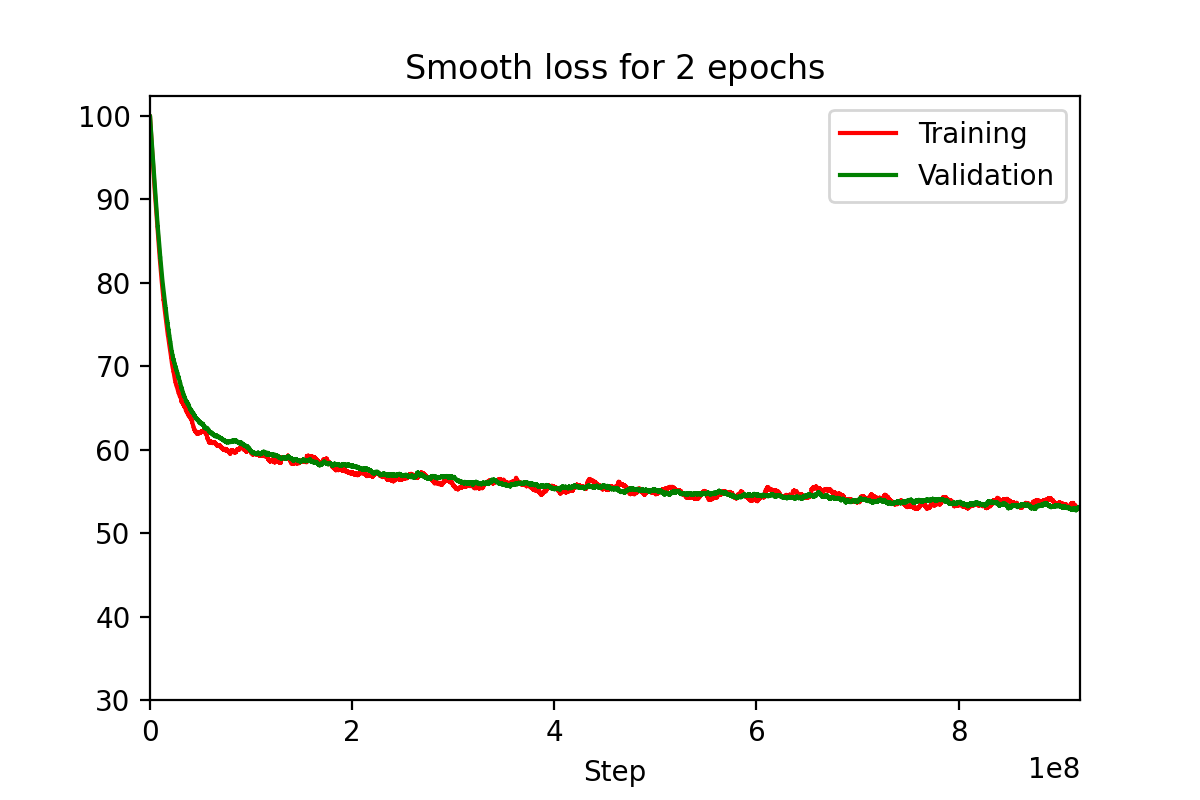
\includegraphics[width=6cm]{../plots/rnn_loss_v3.png}
		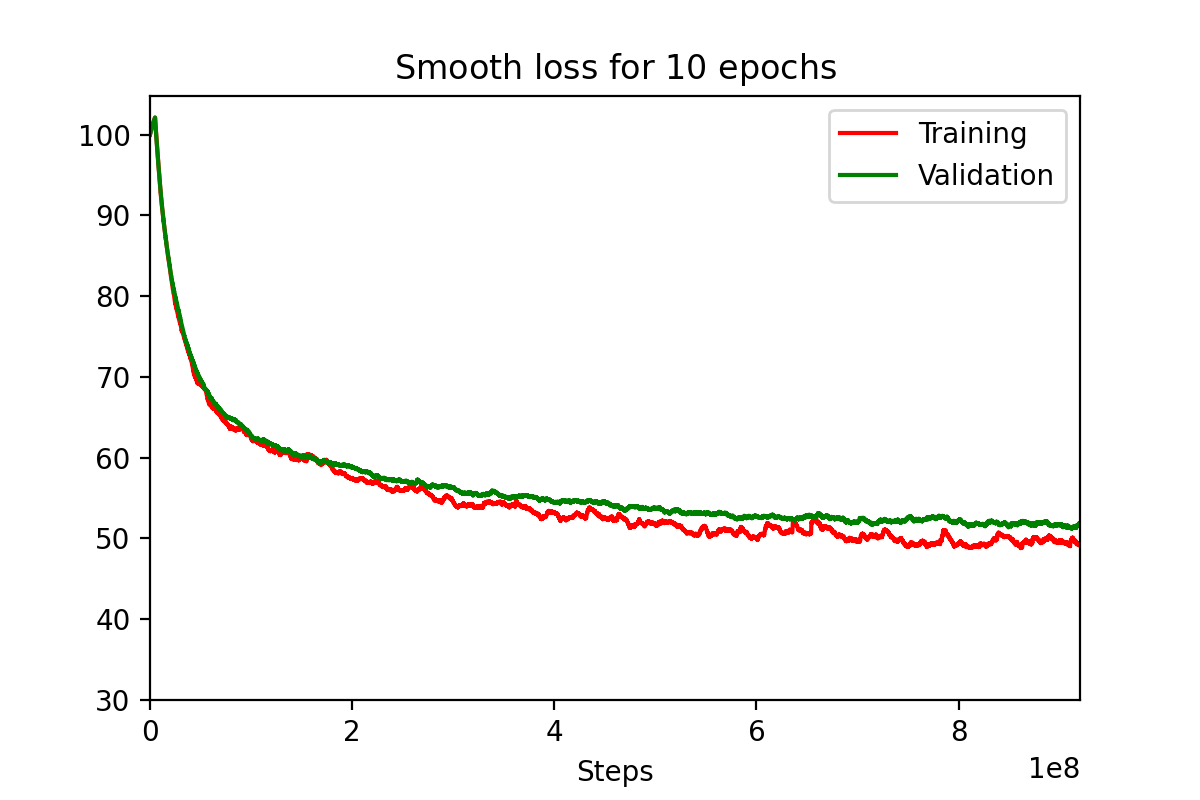
\includegraphics[width=6cm]{../plots/rnn_loss_v4.png}
		\caption{Training and validation loss for \texttt{AdaGrad} (left) and \texttt{Adam} (right), after $2$ epochs of training and $\eta = 0.01$ with randomly ordered blocks of training sequences.}
 	\end{figure}
	The results are more or less identical to those obtained without randomly ordered blocks of training sequences. That is, randomizing the sequences does not seem to improve the ability of the model to learn or to generalize significantly much better to new data. In order to possibly improve this, I train another set of models with $T=50$,  $m = 200$, and using \texttt{He} initialization. All loss metrics have been normalized with respect to the sequence length to allow for a proper comparison. The results do seem to show that is it possible to achieve a lower loss with the combination of randomized blocks sequences, a wider net, \texttt{He} initialization and a longer sequences, e.g. $T = 50$.
	\begin{figure}[h!]
		\centering
		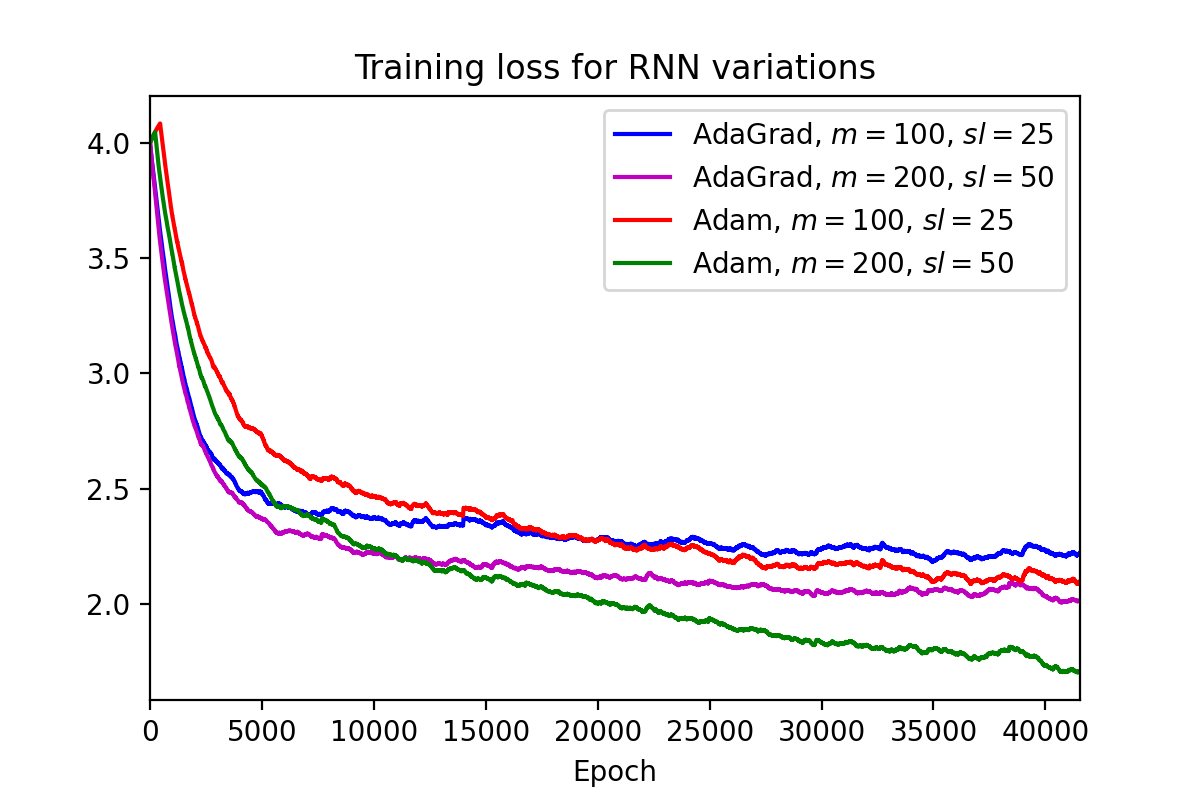
\includegraphics[width=7cm]{../plots/loss_train_comp_rnn.png}
		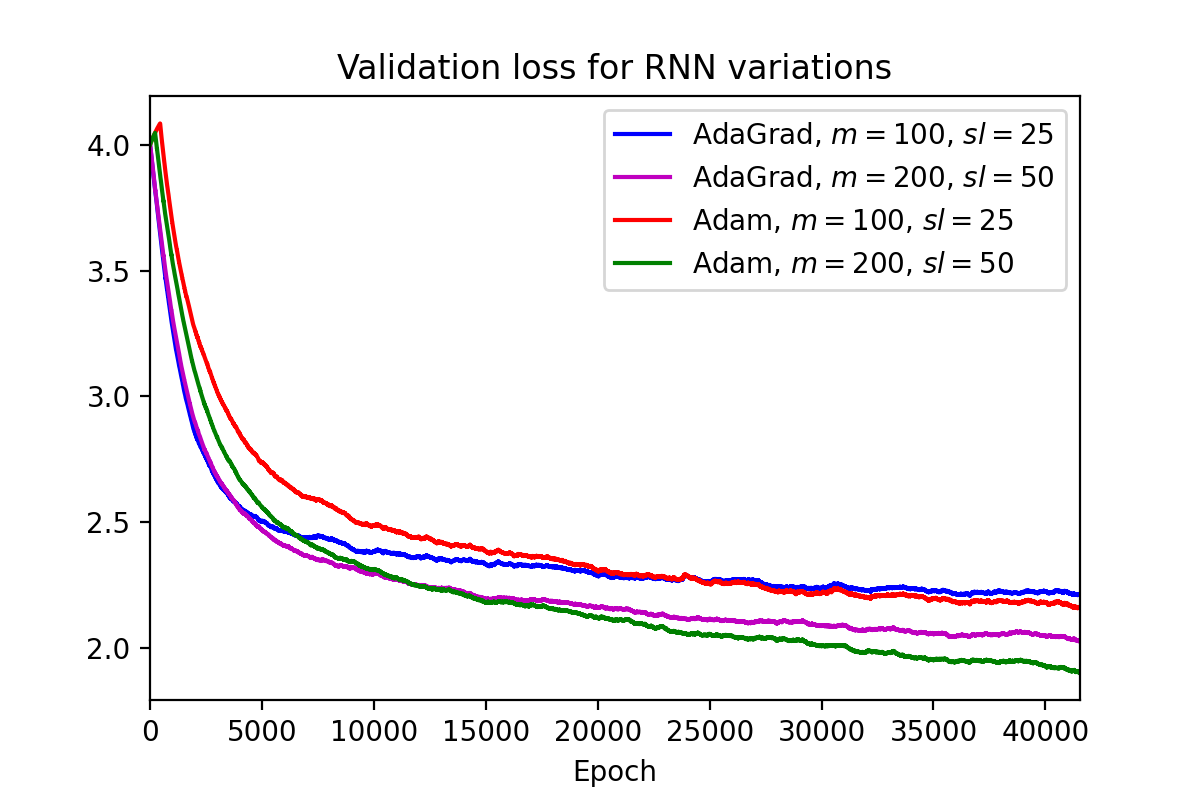
\includegraphics[width=7cm]{../plots/loss_val_comp_rnn.png}
		\caption{Training and validation loss for models trained with randomized blocks with $T \in \{25, 50\}$ and $m \in \{100, 200\}$, and in the case of longer sequences: \texttt{He} initialization.}
 	\end{figure}

\newpage
\subsection*{Generating (more) realistic text sequences}
	First, I drew upon the results from the two previous experiments to train a better model. I chose to pursue a model with \texttt{Adam}, using $T=50$, $m=200$, \texttt{He} initialization and a longer training period: $5$ epochs with $\eta = 0.001$. The training results are displayed in the figure below.
	\begin{figure}[h!]
		\centering
		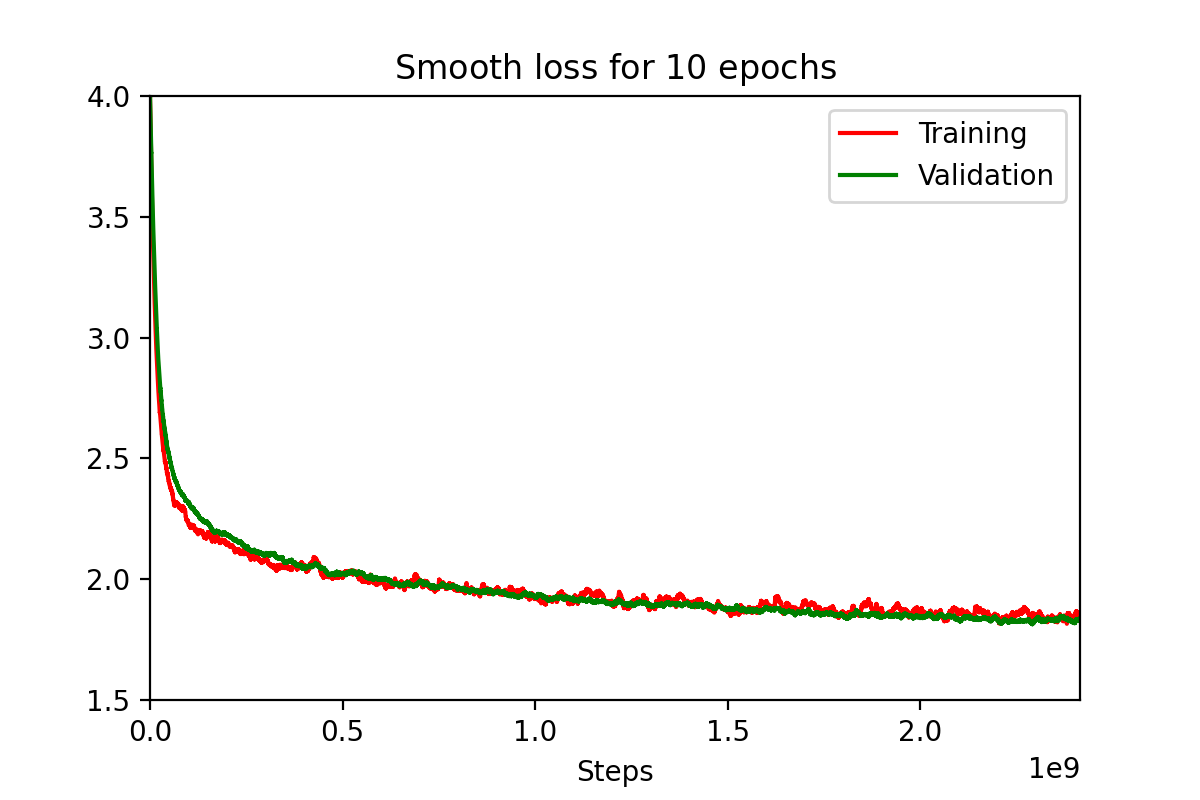
\includegraphics[width=9cm]{../plots/rnn_loss_v7.png}
		\caption{Training and validation loss for \texttt{Adam}, after $5$ epochs of training with $\eta = 0.001$, with $T = 50$ and $m = 200$ with \texttt{He} initialization.}
 	\end{figure}
	In what follows, I will display some examples of generated text when using varying temperature values, $\tau$, and varying thresholds, $\theta$. Since the effects $\tau$ and $\theta$ are in a sense proportional - i.e. a high $\theta$ has an effect similar to that of a hihg $\tau$, and vice versa - I have attempted to separate the effects.

\subsection*{Varying $\theta$}
\subsubsection*{$\tau=1.0$, $\theta=1.0$}
	\begin{quote}
		le and at the said to enchundly all the semplement the gurgon starting of the girnt me the get the suy streakel the seemort the statered the seemed the seetourer to tell the said and the seemed the seemed  near the sehthe should the seem the firstor ke the seemed the stand as the going tarking at the
	\end{quote}

\subsubsection*{$\tau=1.0$, $\theta=0.9$}
	\begin{quote}
		leating the seared as scother and had herely herdly at a fare.  "He pangeonte, his eeglletsed wouldngen hainger to he doom of the would it had sown white go anyou should be a very said, alampurer, and her moget."\\He fillong sor studing as if recerts was trilling to fah than myouse this more a lifttic
	\end{quote}

\subsubsection*{$\tau=1.0$, $\theta=0.7$}
	\begin{quote}
		ly.  walling at the toble fas arried the baight a in the seally side out of the carry least all the sed the gall the tark had a nears was every think and toor who on as they have see while her that was the getter to have a dardide her hard her to make of the hands of the was looked disning were all s
	\end{quote}

\subsubsection*{$\tau=1.0$, $\theta=0.5$}
	\begin{quote}
		ly her leffinting of his head had to anyous her seared at the said, her the gried the gerthing her that he had the rembon her lay stand was and the camainst the stranted to her more the said her some of the seeming out the starting to he said as he had been the fired at the firet her are could and th
	\end{quote}

\subsection*{Varying $\tau$}
\subsubsection*{$\tau=0.9$, $\theta=0.9$}
	\begin{quote}
		le.\\He all, if her have the anys, the wearted actshen thing to stuppester har he was recaing to be a mat the grivill with sum the sel got the not get preater to doward a stat it was right in her nobut the all know hare made come off, it to wand her thin the geater to comed her the been it, her hard i
	\end{quote}

\subsubsection*{$\tau=0.7$, $\theta=0.9$}
	\begin{quote}
		leasing the going to he hear that  and the seally the gainstanting that her the past doing at the rall of the hand that the get and to get the some the stink of a sears the fair the cand Harry could up the was a sere all the back the tors at the still the name at the meally sert to he was something a
	\end{quote}

\subsubsection*{$\tau=0.5$, $\theta=0.9$}
	\begin{quote}
		look it had see on the said, and he was to and came of the fack of the said a manting to the going to the graid to be starter and the seem the bely the perstrough his still as the suind the seemed to he was and the sound the terming the seemed to he was some sereld her the belion of her hear her the
	\end{quote}

\subsection*{Conclusions}
	Varying $\theta$ and $\tau$ clearly have similar effects. As we decrease the parameter values, the generated becomes more "deterministic", and the variation in text decreases rapidly. The model generates fewer special characters and line breaks and the text seems overall to be less "expressive". It seems an "optimal" parameter set is something like $\theta=0.9$, $\tau = 0.7$, in order to generate fairly expressive text containing some keywords and names, such as "Harry". However, the larger problem is that the model has a difficult time generating actual words using character sequences. It seems difficult to get more than marginal improvements from more hidden units and longer sequences when employing an RNN. Rather, it might be necessary to extend the model to e.g. an LSTM or a GRU, which is a kind of "simplified" LSTM. It might also be helpful to employ embeddings instead of the sparse categorical inputs attained from one-hot encoding vectors. 
\end{document}